\documentclass[11pt,a4paper]{report}

\usepackage[spanish]{babel}
%\usepackage[math,light]{iwona}
\usepackage[utf8]{inputenc}
\usepackage{amsmath, amsthm}
\usepackage{amsfonts, amssymb, latexsym}
\usepackage{enumerate}
\usepackage[usenames, dvipsnames]{color}
\usepackage{graphics,graphicx, float} %para incluir imágenes y colocarlas
\usepackage{colortbl}
\usepackage{graphicx}
\usepackage{wrapfig}
\usepackage[top=4cm]{geometry}
\usepackage{cite}
\usepackage[official]{eurosym}
\usepackage{cancel}
\usepackage{subfigure}
\usepackage{tikz}
\usepackage{pseudocode}

\theoremstyle{plain}
\newtheorem{exe}{Ejercicio} % reset theorem numbering for each chapter

\theoremstyle{definition}
\newtheorem{sol}{Solución}

\usepackage[bookmarks=true,
            bookmarksnumbered=false, % true means bookmarks in
                                     % left window are numbered
            bookmarksopen=false,     % true means only level 1
                                     % are displayed.
            colorlinks=true,
            linkcolor=webblue,
            citecolor=red]{hyperref}
\definecolor{webgreen}{rgb}{0, 0.5, 0} % less intense green
\definecolor{webblue}{rgb}{0, 0, 0.5}  % less intense blue
\definecolor{webred}{rgb}{0.5, 0, 0}   % less intense red

\setlength{\parindent}{0pt}
\setlength{\parskip}{1ex plus 0.5ex minus 0.2ex}

\newcommand{\HRule}{\rule{\linewidth}{0.5mm}}

\begin{document}


\begin{titlepage}

\begin{center}

% parte superior de la página
\begin{minipage}{0.4\textwidth}
\begin{flushright}
$\qquad$\htmladdnormallink{
\includegraphics[width=0.25\textwidth]{./ugr}}
      {ugr.es}\\[1cm]
\end{flushright}
\end{minipage}
\begin{minipage}{0.4\textwidth}
\begin{flushleft}
$\qquad$\htmladdnormallink{
\includegraphics[width=0.25\textwidth]{./etsiit}}
      {ugr.es}
\end{flushleft}
\end{minipage}
~\\[1cm]

\textsc{\LARGE Trabajo de Fin de Grado}\\[1.5cm]
\textsc{\Large Escuela Técnica Superior de Ingeniería Informática y Telecomunicaciones}\\[0.5cm]
\textsc{\Large Universidad de Granada}\\[0.5cm]


% título
\HRule \\[0.4cm]
{\huge\bfseries Generación Automática de los Horarios}\\[0.4cm]

\HRule \\[1.5cm]

% autor y supervisor
\begin{minipage}{0.4\textwidth}
\begin{flushleft} \large
\emph{Autor:}\\
\textsc{Braulio Vargas López}\\
\textsc{Marta Gómez Macías}
\end{flushleft}
\end{minipage}
\begin{minipage}{0.4\textwidth}
\begin{flushright} \large
\emph{Supervisor:} \\
Dr.~\textsc{Joaquín Fernández Valdivia}
\end{flushright}
\end{minipage}

\vfill

% parte inferior de la página
{\large \today}

% \vspace{5mm}

%       %\footnotesize
%       \htmladdnormallink{
\includegraphics[width=2cm]{88x31.jpg}}
%       {http://creativecommons.org/licenses/by-nc-sa/3.0/}\\
%       \texttt{Lecciones sobre Orientación by 
%       \href{mailto:mi_direccion@hotmail.com}{L. Vargas}
%       is licensed under a \htmladdnormallink{Creative Commons
%       Reconocimiento-NoComercial-CompartirIgual 3.0 Unported License}
%       {http://creativecommons.org/licenses/by-nc-sa/3.0/}
%       Permissions beyond the scope of this license may be available at
%       \htmladdnormallink{L. Vargas}{http://www.mi_web.com}}.

\end{center}

\end{titlepage}

\tableofcontents

% Descripción de sistemas "privativos"

\chapter{Descripción de otros sistemas software similares}

\section{Lantiv Scheduling Studio}

El software llamado \href{http://www.schedulingstudio.com/}{\textit{Lantiv Scheduling Studio}} es una herramienta para realizar horarios de forma \textbf{no automatizada}. Permite usar variables tales como profesorado, número de alumnos, aulas o equipamiento y, al realizar una modificación en el horario realizado, confirma que no hay ninguna incompatibilidad.

Permite realizar un calendario semanal, bisemanal o programar actividades para días concretos. Además, también permite elegir las horas a las que empieza y acaba cada actividad y, por último, también permite programar los descansos y su duración.

Respecto a su interfaz, permite cambiar el idioma y la combinación de colores que ésta usa. Al ser un programa genérico, incluye herramientas y ejemplos para hacer horarios en todo tipo de instituciones. El software puede configurarse para trabajar en un servidor (usando la IP y el puerto del mismo, además de un usuario y una contraseña), de manera que todas las personas que trabajen sobre el mismo horario puedan ver los cambios que se realizan en éste en tiempo real.

Toda esta información puede encontrarse en la documentación del software \cite{lantiv}.

\section{Mimosa}

El software llamado \href{http://www.mimosasoftware.com/}{\textit{Mimosa}} es una herramienta para realizar horarios de forma \textbf{automatizada}. A partir de información que el usuario debe introducir a mano, este software genera un horario usando algoritmos de optimización. Dicha información es: clases, profesores, salas especiales, equipo, asignaturas y alumnos. 

En la \hyperref[mimosa]{Figura \ref*{mimosa}} vemos varios pantallazos de su interfaz en la que hay varias áreas principales: una para introducir la información relativa al horario (referida en el software como \textit{recurso}), otra para añadir las asignaturas y una para ver los horarios creados. En ésta última sección podemos filtrar el horario por grupo, profesor o aula.

\begin{figure}[!h]
    \centering
    \mbox {
    \subfigure[Sección de recursos]{
    \label{recursos}
    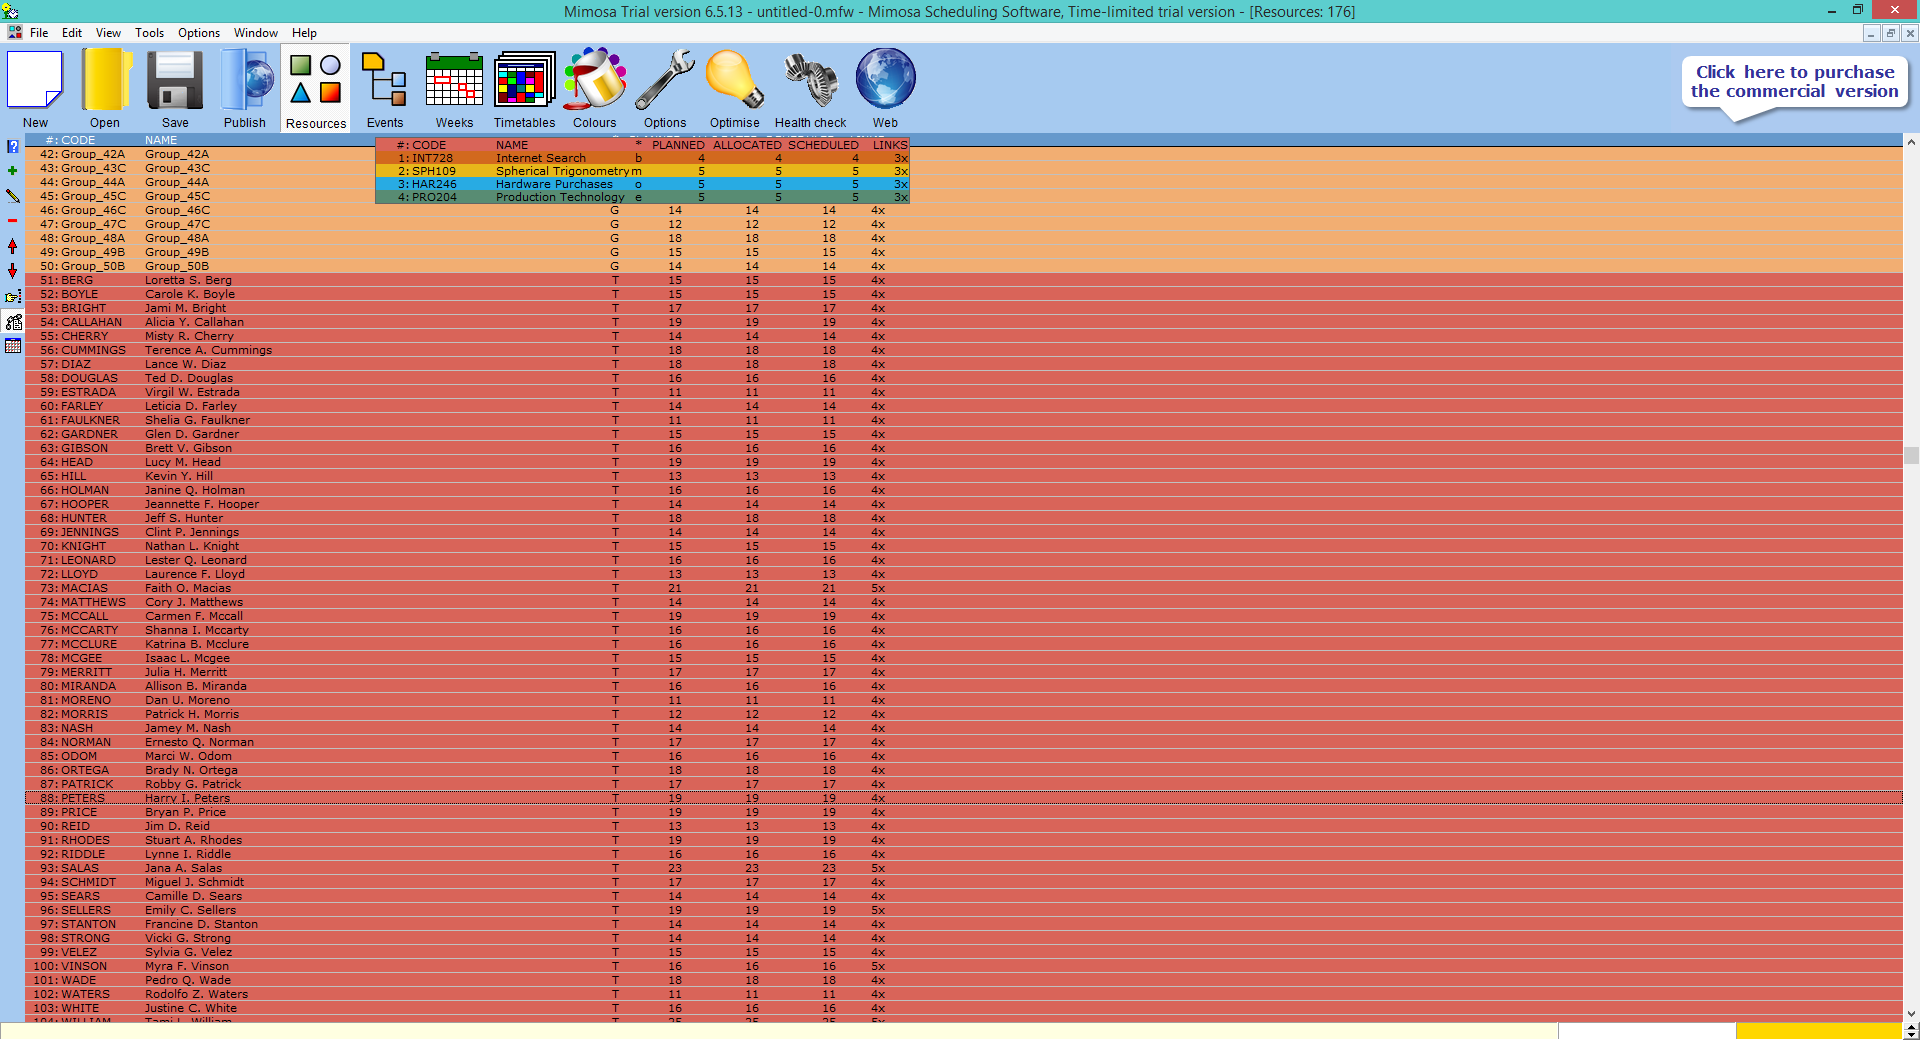
\includegraphics[width=0.5\textwidth]{1}
    }
    \qquad
    \subfigure[Sección de asignaturas]{
    \label{eventos}
    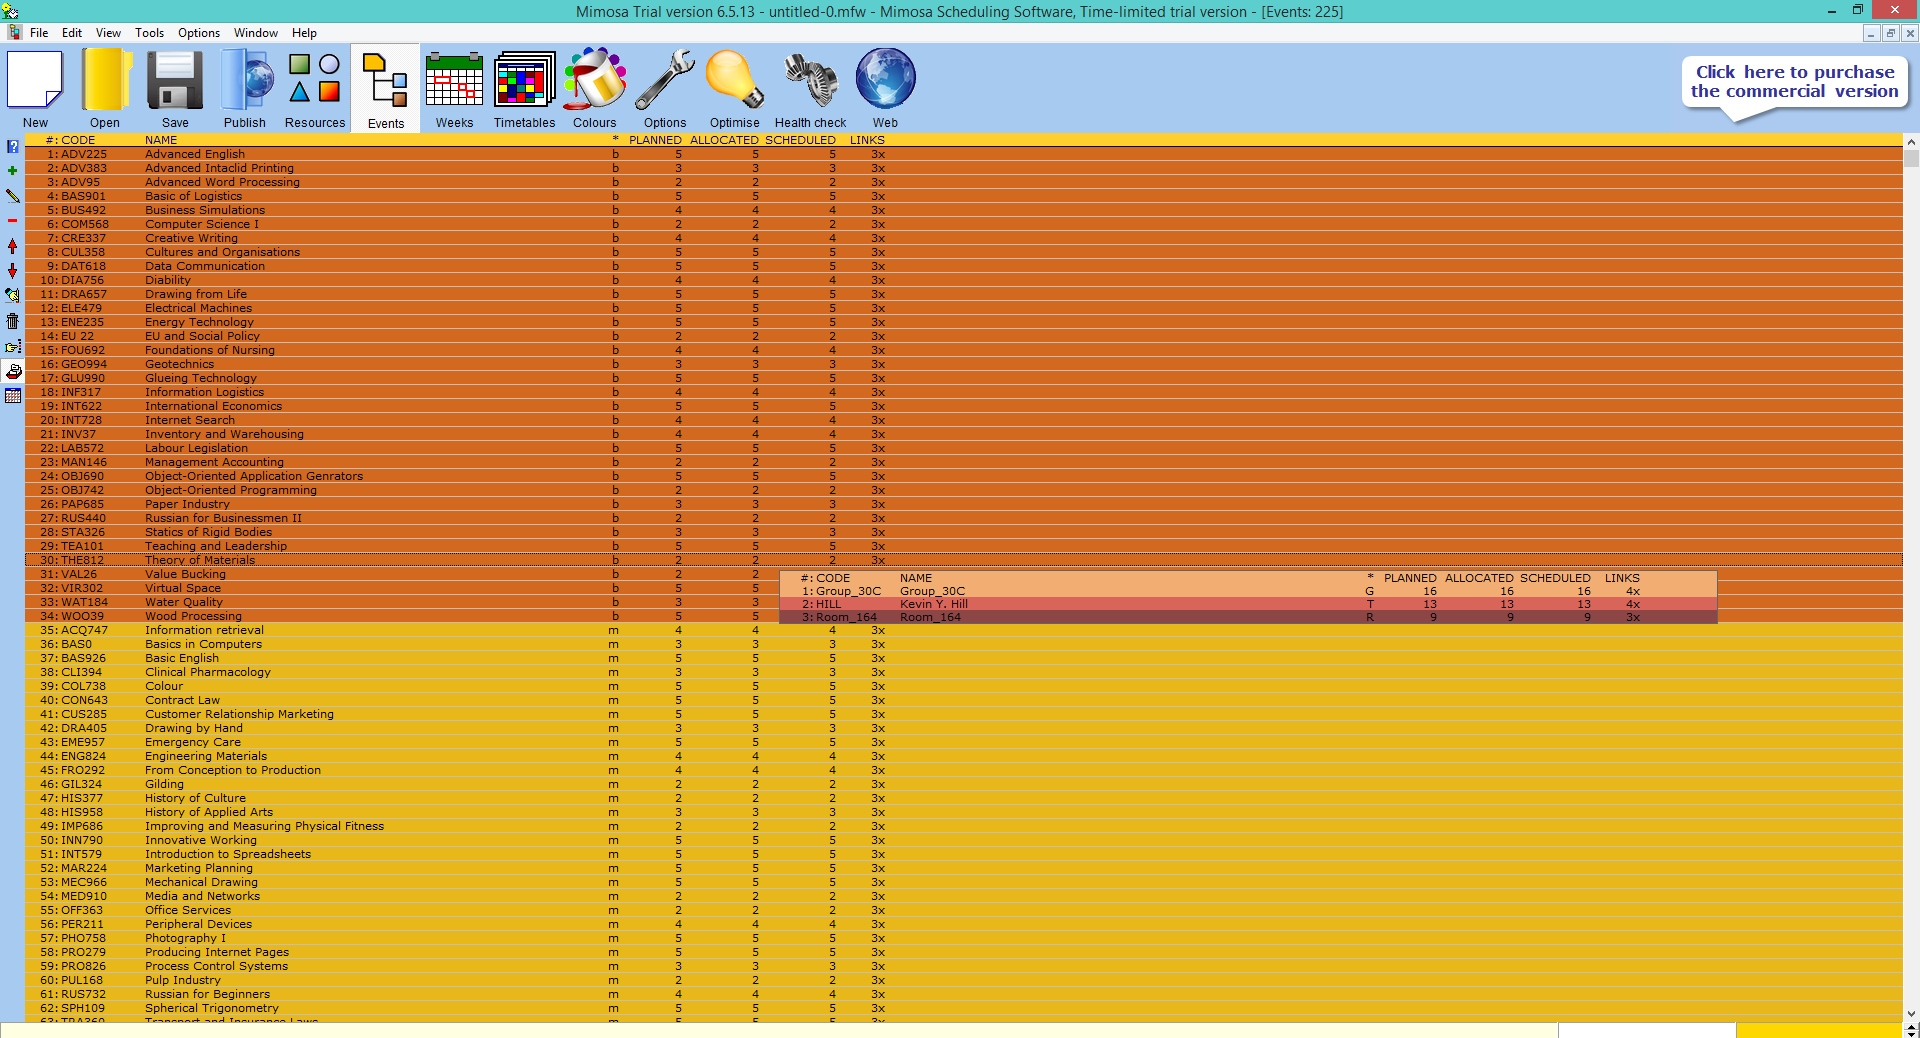
\includegraphics[width=0.5\textwidth]{2}
    }
    }
    \subfigure[Sección de horarios, en la que hemos filtrado el grupo 29C] {
    \label{tabla}
    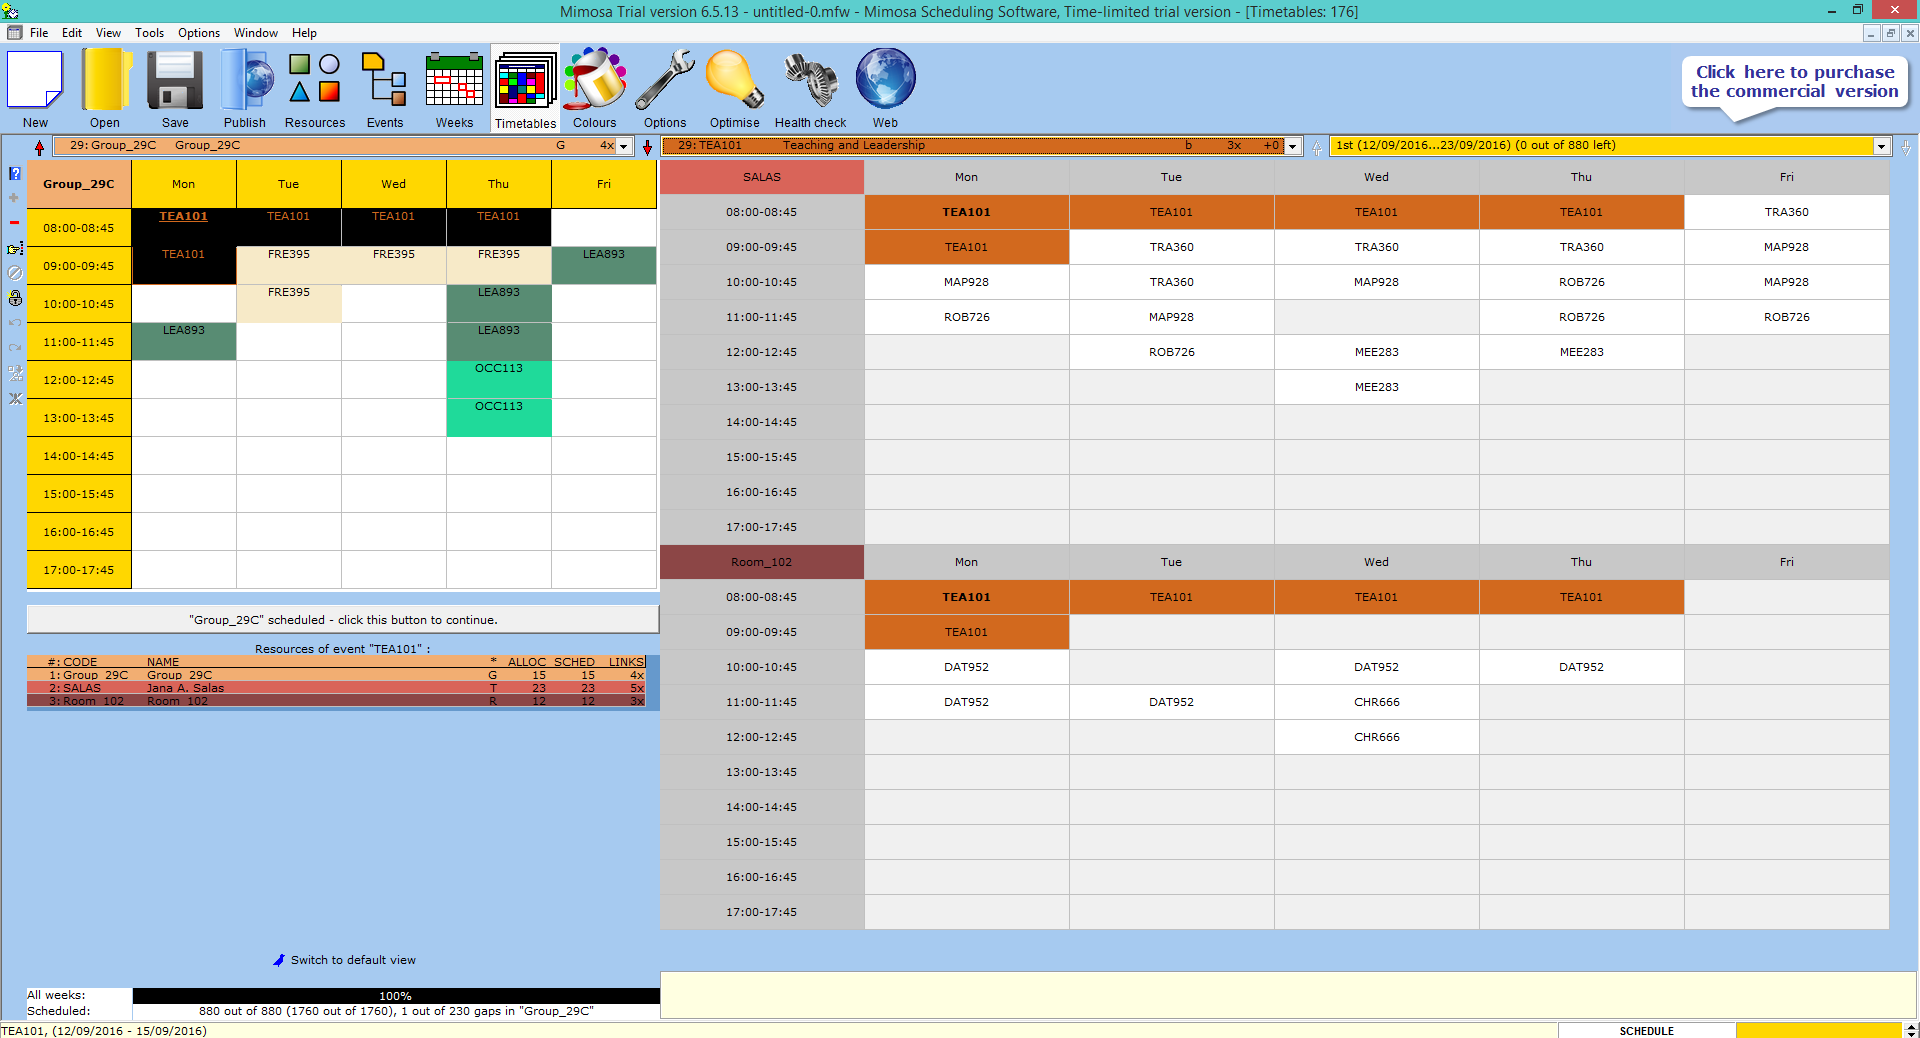
\includegraphics[width=0.5\textwidth]{3}
    }
    \caption{Capturas de pantalla del software \textit{Mimosa}}
    \label{mimosa}
\end{figure}

Por último, \textit{Mimosa} permite exportar el horario generado en distintos formatos tales como \texttt{csv} o web y además de realizar un horario, también permite asignar profesores y alumnos a cada grupo de forma automatizada.

Toda esta información se puede encontrar en su documentación \cite{mimosa}.

\section{Timetabler}

El software llamado \href{http://www.timetabler.com/}{\textit{Timetabler}} es una herramienta para realizar horarios tanto de forma \textbf{no automatizada} (modo interactivo) como de forma \textbf{automatizada}. Incluso permite mezclar ambas, permitiendo que el software realice un horario y el usuario resuelva a mano las posibles incidencias que éste encuentre.

Su modo de funcionamiento se basa en realizar cuatro pasos de forma secuencial:

\begin{enumerate}[1.]
    \item \textbf{Basic data}: en primer lugar, se introduce el profesorado (además del departamento en el que está) y su disponibilidad, los grupos en los que se va a dividir al alumnado, las aulas, las asignaturas a impartir y la estructura del horario (horas en las que se va a dar clase y descansos, días de la semana en los que se va a dar clase, etc). Esta información también puede ser \textbf{importada} desde un fichero.
    \item \textbf{Activities}: a continuación, se describe cada asignatura en términos del número de horas que será impartida. Además, permite ver un resumen de todos los datos introducidos hasta el momento.
    \item \textbf{Schedule}: en este paso, se realiza el horario. Podemos hacerlo de tres formas: manual, semi-automático y automático. 
    \item \textbf{Print}: por último, podemos imprimir el horario en base a una asignatura, un grupo académico, un profesor o un aula. Además, podemos exportar las tablas en distintos formatos y realizar una copia de seguridad.
\end{enumerate}

Una descripción detallada de estos cuatro pasos puede encontrarse en \cite{timetabler}.


% Descripción de sistemas "libres"

\chapter{Otros proyectos libres similares}

A continuación podremos ver algunos de los proyectos que podemos encontrar por \textit{\textbf{Github}} sobre la generación automatizada de horarios.

\section{Plan}

\href{https://github.com/adamcik/plan}{\textit{Plan}} es un software desarrollado como asistente para la creación de horarios de una forma fácil para los estudiantes de \textit{NTNU}, tal y como se puede ver en \cite{plan}.

Esta interfaz web nos pide que creemos un \textit{nick} para poder entrar en la aplicación. Una vez creado, nos pasará a la interfaz que vemos en la \hyperref[plan1]{Figura \ref{plan1}}

\begin{figure}[H]
    \centering
    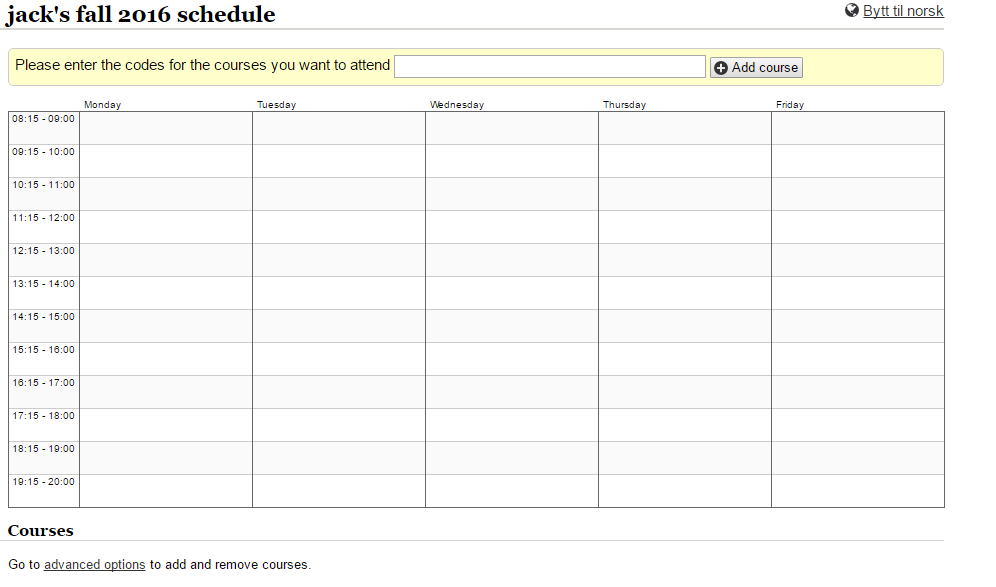
\includegraphics[width=0.7\textwidth]{plan1}
    \label{plan1}
    \caption{Interfaz web para la introducción de las asignaturas}
\end{figure}

En esta interfaz web, tendremos que ir introduciendo los códigos de las asignaturas, generando una tabla de asignaturas en la que el alumno se habrá matriculado, tal y como se puede ver en la \hyperref[plan2]{Figura \ref{plan2}}. En esta tabla, aparecerán los códigos de las asignaturas, su descripción, su fecha de examen y ofrece la posibilidad de dar un alias a la asignatura.

\begin{figure}[H]
    \centering
    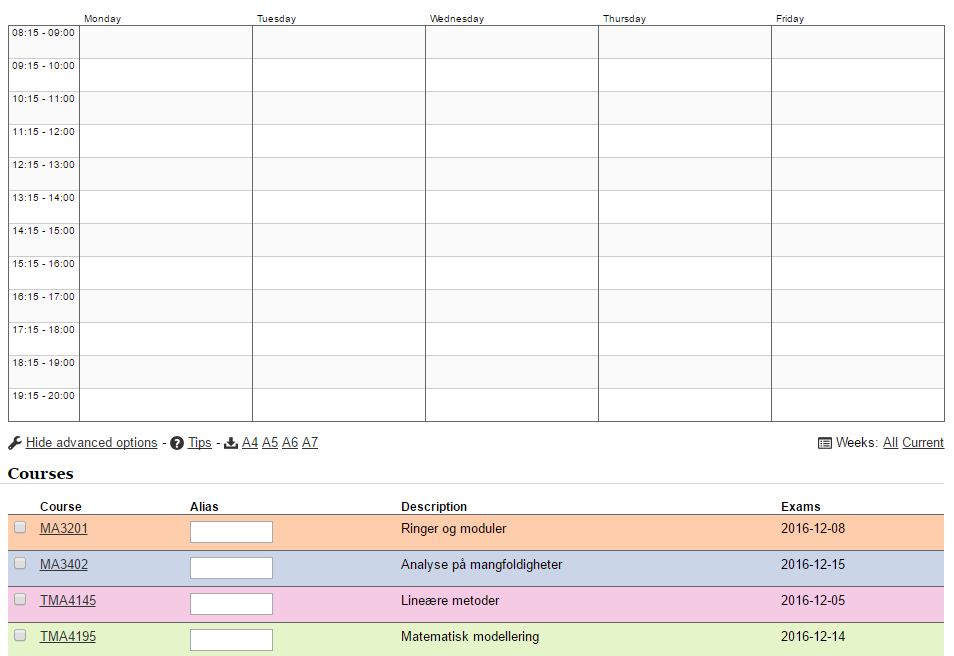
\includegraphics[width=0.7\textwidth]{plan2}
    \label{plan2}
    \caption{Tabla de asignaturas introducidas con sus respectivos códigos}
\end{figure}

Una vez introducidas, el alumno seleccionará los grupos en los que está matriculado y el sistema mostrará automáticamente \textbf{el horario específico para el alumno}. Es decir, dado un alumno con un conjunto de asignaturas $\mathcal{X}$, el sistema mostrará el horario que tiene el alumno en cuestión, como vemos en la \hyperref[plan3]{Figura \ref{plan3}}. A su vez, el sistema ofrece una lista con las clases de cada asignatura y grupo más detallada, como se ve en la \hyperref[plan4]{Figura \ref{plan4}}


\begin{figure}[H]
    \centering
    \mbox {
        
        \subfigure[Horario generado.]{
            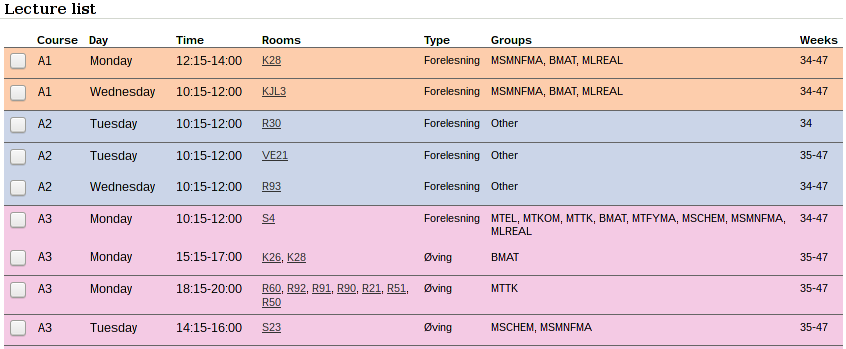
\includegraphics[width=0.5\textwidth]{plan3}
            \label{plan3}
        }
        
        \quad
        
        \subfigure[Lista más detallada de las clases del día.] {
            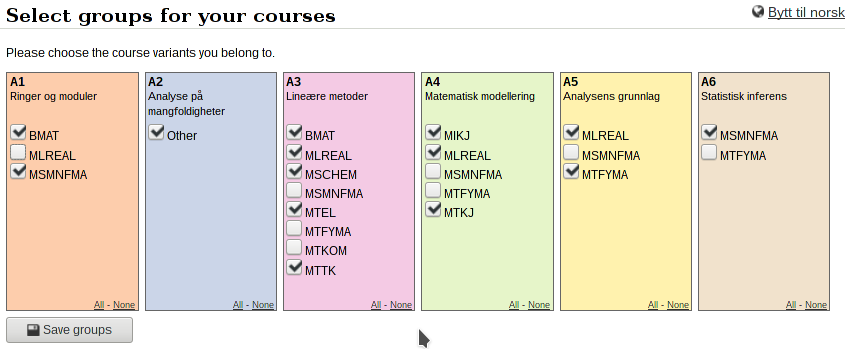
\includegraphics[width=0.5\textwidth]{plan4}
            \label{plan4}
        }
    }
    
    \caption{Horarios y listas que genera el sistema}
    \label{plan3-4}
\end{figure}

Este software ofrece actuálmente varias funciones tales como:

\begin{enumerate}
	\item Una vista personificable del calendario.
	\item Se puede exportar fácilmente a \textit{Google-Calendar}.
	\item Se puede imprimir en formato PDF.
	\item El usuario puede decidir las horas límites.
	\item Permite importar información sobre las asignaturas mediante volcados de una base de datos.
\end{enumerate}

\section{Timetable Generator}

\href{https://github.com/zeus9/timetable_generator}{\textit{Timetable Generator}} es un generador de horarios desarrollado por el usuario \textbf{zeus9} de \textit{Github}. Está desarrollado en C++ y Python 2, haciendo uso de un algoritmo genético para la generación del horario, tal y como se puede ver en \cite{timetableGenerator}.

Este sistema toma como entrada tres ficheros en formato \textbf{\textit{CSV}}, en los que se incluye la siguiente información:

\begin{enumerate}[$\bullet$]
    \item \texttt{initial.csv}: consiste en un fichero que contiene una matriz inicial que conforma el horario. Este horario inicial se utiliza en el algoritmo genético del fichero \textit{labGa.cpp}.
    \item \texttt{periodcount.csv}: supone una relación entre los $ID's$ de los profesores, disponibles en \textit{faculty.csv} y algo más aún por descifrar.
    \item \texttt{labPeriodcount.csv}
\end{enumerate}

Todo esto conforman los datos mínimos de la universidad que necesita el algoritmo para generar el horario. 

Para ejecutar el algoritmo, tiene que ser bajo una distribución Linux, y se realiza ejecutando en un terminal \texttt{./ttgen.sh}. Con esto, aparecerá en pantalla una interfaz muy simple que nos permite configurar los parámetros de ambos algoritmos como se ven en la \hyperref[ttgen1]{Figura \ref{ttgen1}}.

\begin{figure}[H]
    \centering
    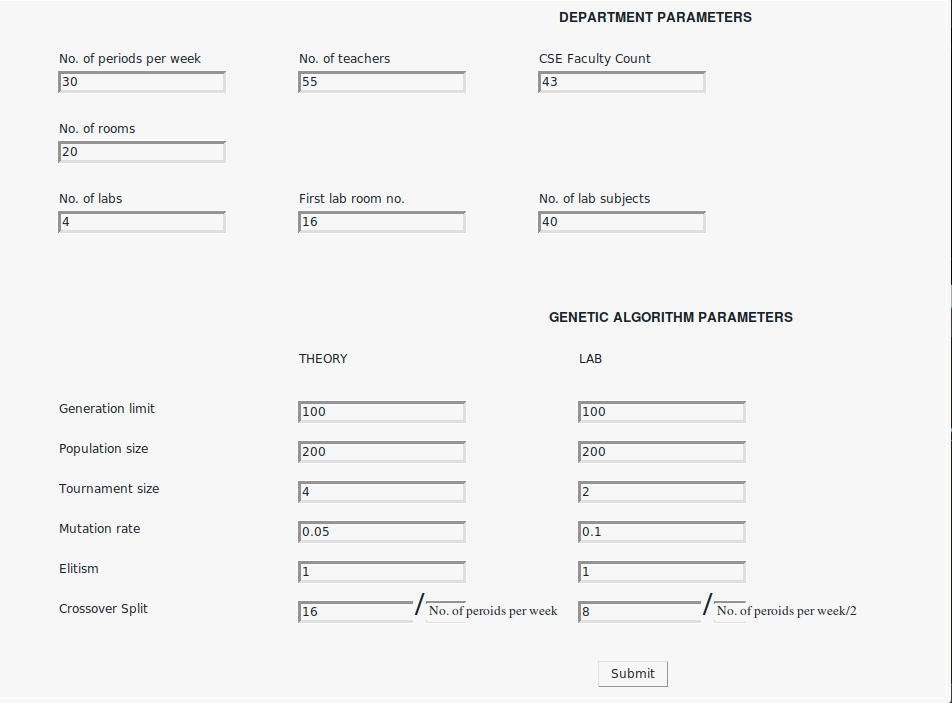
\includegraphics[width=0.7\textwidth]{ttgen1}
    \label{ttgen1}
    \caption{Interfaz para modificar los parámetros del algoritmo genético}
\end{figure}

Tras modificar los parámetros del algoritmo y pulsar el botón \textit{Submit}, estos datos se escriben en el fichero \textit{variables.csv} para el algoritmo genético de \textit{ga.cpp} y en \textit{labVariables.csv} para el algoritmo de \textit{labGa.cpp} y se comienza a ejecutar el $script$ en Python \texttt{labConflictsGen.py} que genera un CSV con las incompatibilidades que pueda haber en las aulas.

A continuación, se ejecuta el algoritmo genético. La variante \texttt{labGa} comienza con un horario inicial de entrada, dando pie al algoritmo genético, a diferencia de \texttt{ga}, que comienza sin un horario de entrada. Al finalizar, ambos muestran por la terminal la solución encontrada, y el coste de esta, siendo a su vez escrito en un fichero.

\section{Unitime}

\href{https://github.com/UniTime/unitime}{\textit{UniTime}} es un sistema que se acerca mucho al sistema deseado, ya que integra un sistema para la generación del horario, asignación de aulas, asignación de exámenes$\ldots$ Permita además modificar la estructura del horario y minimiza los conflictos que existen en el horario.

Este sistema, disponible en \cite{unitime}, está desarrollado en Java, y ofrece una interfaz web simple y con facilidad para moverse entre las opciones.

Este sistema ofrece varios niveles de usuario, partiendo desde un alumno hasta un administrador, con distintos niveles de permisos y acciones, siendo este último el que más acciones disponibles tiene, como son añadir asignaturas, departamentos, aulas y edificios, grupos de estudiantes, etc. 

Además de todo esto, el sistema ofrece una amplia documentación en su página web \href{http://help.unitime.org/}{\textit{http://help.unitime.org/}}, junto con una demo de cada uno de los usuarios posibles que tiene el sistema, para poder probar y ver cada una de las funciones de las que dispone el sistema.

Una característica del sistema es que utiliza internamente un algoritmo de búsqueda local para la satisfacción de restricciones. Este algoritmo consiste en una búsqueda hacia delante iterativa, similar a una búsqueda local, pero con la peculariadad de que el algoritmo puede dar soluciones que no satisfazcan todas las restricciones. Es decir, las restricciones se dividen en restricciones fuertes y restricciones débiles. El algoritmo, satisface todas las restricciones fuertes, pero, las restricciones débiles pueden no ser satisfechas, por lo que el algoritmo explora mejor el espacio de búsqueda obteniendo mejores soluciones, más fáciles de entender para el usuario y con la posiblidad de detener el algoritmo en cualquier momento y devolver una solución al ser iterativo.

% Descripción del sistema

\chapter{Descripción del sistema y requisitos}

\section{Descripción del sistema}

La idea general del sistema es ofrecer una forma automatizada de hacer los horarios de una escuela o facultad en base a restricciones tales como el profesorado y su disponibilidad, las aulas disponibles teniendo en cuenta su capacidad y el equipo del que disponen, el número de alumnos de una asignatura, bloques horarios, etc. 

Con este sistema podrán estudiarse distintas propuestas de horarios para maximizar el uso de las aulas, el rendimiento de todo el equipo de una facultad y facilitar el trabajo que supone la creación de un horario para cada nuevo curso.

\section{Objetivos principales del sistema}

\begin{enumerate}[OBJ-1]
    \item El usuario debe introducir la menor información posible para que le resulte más cómodo y sencillo hacer uso del sistema. Esto sería posible si la mayoría de información necesaria para la generación del horario fuera posible obtenerla de la base de datos de la escuela o de la UGR, para evitar que el usuario tenga que realizar ninguna entrada desde ficheros o similares.
    
    \item Tener la posibilidad de realizar un nuevo horario desde cero a partir de los datos disponibles, y la posibilidad de, a partir de uno ya generado, generar uno nuevo a partir de modificaciones.

    \item Sobre la solución del sistema, existen dos opciones:
    \begin{enumerate}[a)]
        \item Ofrecer una única solución y ofrecer la posibilidad de realizar modificaciones sobre esta de forma interactiva y que el sistema avise de posibles conflictos.
        \item Ofrecer como salida un parapeto de soluciones que haya encontrado el sistema y que el usuario final elija entre las soluciones que más le interesen.
    \end{enumerate}
    % \item Poder conectarse a las bases de datos de la universidad de forma que el usuario introduzca la menor información posible.
    % \item Poder crear un horario válido desde cero usando los datos disponibles.
    % \item Una vez hecha una propuesta de horario, realizar modificaciones sobre la misma de forma que se obtenga un horario válido.
\end{enumerate}

\section{Requisitos del sistema}

\begin{enumerate}[REQ-1]
    \item No pueden solaparse dos asignaturas el mismo día y a la misma hora en el mismo aula.
    \item Cómo máximo hay tres subgrupos de prácticas. Puede haber asignaturas en las que haya dos subgrupos y otras en las que haya sólo uno.
    \item Para cada grupo se debe de decidir de forma manual su franja horaria y el aula de teoría.
    \item No puede haber más de tres grupos de teoría asignados al mismo aula en el mismo turno (mañana o tarde). 
    \item Se debe saber de antemano el número de horas de teoría y prácticas de cada asignatura.
    \item Si el número de horas de teoría o prácticas de una asignatura es impar, se agrupará con otra asignatura que esté en la misma situación. En caso de que no sea posible, ésta hora se añadirá al principio o al final del turno ofreciendo la posibilidad de cambiarla manualmente.
    \item Se debe dar la posibilidad de para una asignatura, dar las horas de teoría en un mismo turno de dos o más horas, o repartir las sesiones de teoría a lo largo de la semana en días distintos.
    \item El horario obtenido para cada grupo no debe de contener huecos, es decir, debe ser lo más compacto posible.
    \item Las distintas especialidades tienen su horario en paralelo para no favorecer ninguna especialidad sobre otra.
    \item Se debe registrar el equipamiento disponible en cada laboratorio y el que cada asignatura necesita para llevar a cabo sus prácticas de forma que el sistema realice la asignación a laboratorios de forma automática.
    \item Se debe poder elegir el número de días y la franja horaria para cada titulación por separado. 
\end{enumerate}


%% Bibliografía y referencias
\bibliography{bibliografia.bib} %archivo citas.bib que contiene las entradas 
\bibliographystyle{siam} % hay varias formas de citar
\end{document}
